% !TEX root = ../thesis.tex

% Tässä osassa kuvataan käytetty tutkimusaineisto ja tutkimuksen metodologiset valinnat, sekä kerrotaan tutkimuksen toteutustapa ja käytetyt menetelmät.

% http://en.wikipedia.org/wiki/YUV#Y.27UV420p_.28and_Y.27V12_or_YV12.29_to_RGB888_conversion
% https://msdn.microsoft.com/en-us/library/windows/hardware/ff538197%28v=vs.85%29.aspx

% MITATTAVIA SUUREITA!

\documentclass[thesis.tex]{subfiles}

\begin{document}

\chapter{Design and Implementation}
\label{chapter:design-implementation}

\section{Requirements}

The goal of the thesis was to investigate if it were feasible to utilize smartphone technology to analyze photoluminescent material for product authentication purposes. The example use case was to have a smartphone application that would be able to identify products tagged with a chemical marker (taggant) as being either fake or authentic. This required implementing a smartphone application that could satisfy the following requirements (requirements \ref{R2} and \ref{R3} refer to the actual product authentication process, whereas \ref{R1} and \ref{R4} are additional feature requirements):

\begin{enumerate}[leftmargin=0.55in, label=\textbf{R\arabic*}]
	\item \label{R1} Support the Windows Phone platform (preferably cross-platform)\\ \\
	Windows Phone was chosen as the initial target platform based on the Lumia 1020 smartphone, which was allocated for the project and featured one of the best smartphone cameras on the market. An additional goal was set for supporting other major platforms (Android and iOS) in the hopes of being able to compare the results across vendors.

    \item \label{R2} Capture the emission of a luminophore as a function of time\\ \\
    It was outlined that the application should be capable of capturing the emission of a taggant (luminophore) as a sequence of images at pre-defined intervals that should not exceed 1000ms. The sequence of captured images would work as a unique \emph{fingerprint}. Implementation details, such as the capture method (video vs. images), capture properties (e.g. ISO) or properties of the light source (e.g. wavelength, luminance) were not separately specified.
    % - in relation to Q1

    \item \label{R3} Use the capture data (fingerprint) to query a remote product catalog\\ \\
    The use case (product authentication) required that the fingerprint could be linked to a physcial object, e.g. a product. The requirement here was twofold: given a pre-defined database of fingerprints and products (1) characterize the capture data as a fingerprint and (2) match it against the existing fingerprints to find the corresponding product in a remote product database. In case of a match, the user's geolocation should also be stored for further verification and analytics purposes.

	\item \label{R4} Support (secure) offline usage\\ \\
	Implementing support for offline usage was seen as an attractive feature that would differentiate the application from the competition. It would also allow investigating the feasibility of storing data client-side from a security and storage strategy perspective.
\end{enumerate}

\noindent The following chapters discuss these requirements further and present the related implementation details. The implementation for \ref{R2} and \ref{R3} is presented in Chapter \ref{chapter:fingerprint-pipeline}. Requirements \ref{R1} and \ref{R4} are discussed in Chapters \ref{chapter:application-architecture} and \ref{chapter:storage-security}, respectively.

\section{Application Architecture}
\label{chapter:application-architecture}

The general architecture of the LuminoTrace application is depicted in Figure \ref{figure:architecture}. The camera application and the external camera module work in tandem to capture and analyze the taggant (luminophore) to construct a fingerprint. To find a product linked to the fingerprint a request is sent over the network to the application server, which queries the databases for a possible match. Alternatively, if the network is unavailable the application will fallback to querying a local, filtered copy of the database. Finally, the result of the search is rendered in the UI.

\begin{figure}[h]
\centering 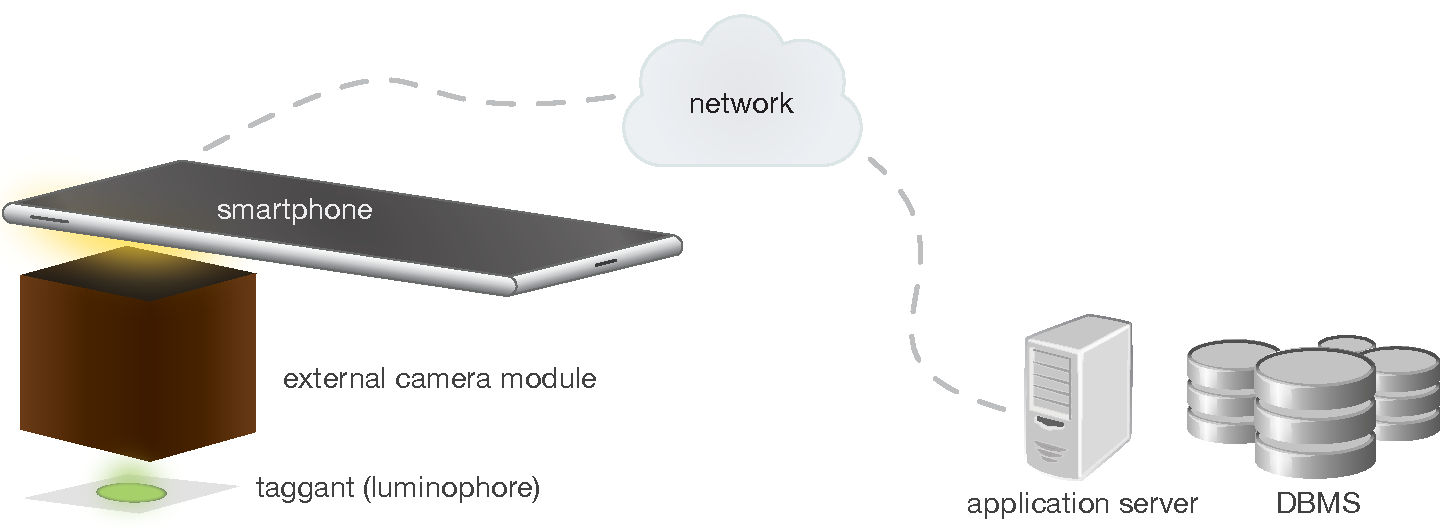
\includegraphics[width=13.5cm]{images/design_implementation/architecture.pdf}
\caption{The general architecture of the LuminoTrace application. \label{figure:architecture}}
\end{figure}

\subsection{Camera Application}
\label{chapter:camera-application}

The camera application was built as a WebView application using Apache Cordova (4.2.0) and Ionic (1.0.0-beta.14). This allowed supporting multiple platforms with minimal effort as the UI and parts of the application logic could be easily re-used across platforms. Furthermore, no platform-specific knowledge was required to implement the UI allowing focus to be kept on the business logic. Android and Windows Phone were chosen as the target platforms. Support for Android was implemented due to the author's previous experience of the platform and the better debugging tools, which both allowed developing the first prototype faster.

Figure \ref{figure:user_interface} presents the user interface. For brevity, the landing page and the two sidebar views (\emph{Past traces} and \emph{Settings}) are combined into a single image and other views, such as success and error pages, are omitted.

\begin{figure}[h]
\centering 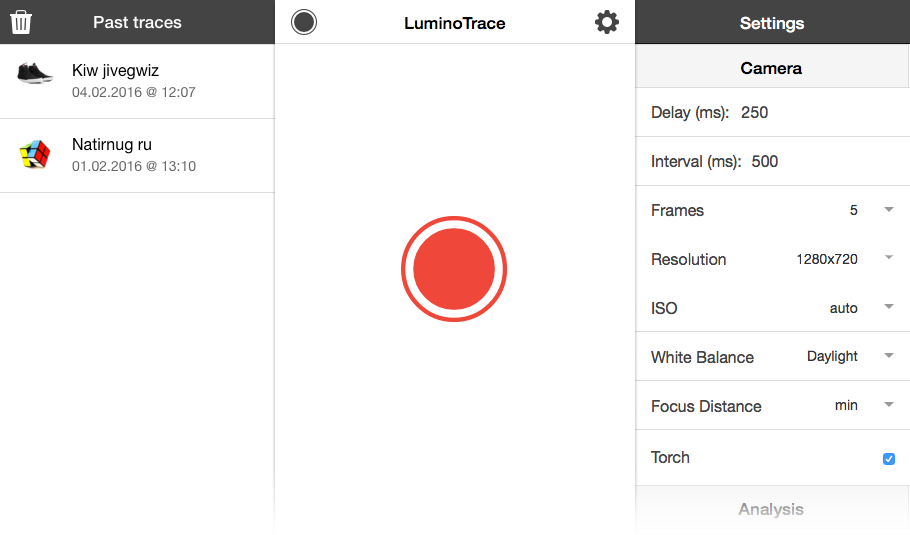
\includegraphics[width=13.5cm]{images/design_implementation/user_interface}
\caption{The user interface of the LuminoTrace application. \label{figure:user_interface}}
\end{figure}

The \emph{Past traces} view displays a history of successfully matched products and allows the user to navigate further to view the relevant product information (e.g. product description and link to an online marketplace). The \emph{Settings} sidebar mainly consists of parameters for configuring the underlying algorithms and the smartphone's camera. These settings were only exposed for research and development purposes and would not be displayed to the end-user in the actual application. The main interaction endpoint for the user is the red capture button on the landing page, which once tapped on, initiates the fingerprint capture process. The captured fingerprint is then analyzed by the application to determine whether or not the given taggant matches a record in the database. This process is discussed in more detail in Chapter \ref{chapter:fingerprint-pipeline}.

To interact with the native Android and Window Phone camera APIs a custom Cordova plugin was implemented. Existing Cordova camera plugins or native 3rd party camera libraries could not be utilized as a more granular control of the output image data was required. The parameters configured and passed to the underlying camera APIs are listed in Table \ref{table:camera-parameters}. Other relevant camera parameters were either disabled (exposure compensation and flash mode) or set to their logical default value (e.g. zoom level of 0). Shutter speed and lens aperture could not be configured due to the lack of support by the API and the hardware, respectively.

\begin{table}[ht]
	\caption{Camera parameters supported by the LuminoTrace application.} \label{table:camera-parameters}

	\begin{center}
	\begin{tabular}{| m{2.75cm} | m{9.75cm} |}

		\hline
		\textbf{Parameter}	& \textbf{Description and Supported Values} \\ \hline
		Delay				& Time to wait before starting capture (0-1500ms) \\
		\hline
		Interval 			& Time between subsequent frames (60-1500ms) \\
		\hline
		Frames 				& Number of frames to capture (1-7) \\
		\hline
		Resolution 			& Capture frame resolution (640x480, 1280x720 or max\footnotesize{*}) \\
		\hline
		ISO 				& ISO sensitivity (100, 200, 400, 800, 1600 or auto) \\
		\hline
		White Balance		& White balance preset to use (daylight or auto) \\
		\hline
		Focus Distance		& Distance to which to set the focus to (min or max) \\
		\hline
		Torch 				& Toggle the torch to trigger the camera module (on/off) \\
		\hline
	\end{tabular}
	\end{center}
	\scriptsize{*} \small{\emph{min} and \emph{max} refer to the minimum/maximum value supported by the platform}
\end{table}

For capturing the fingerprint the application utilizes an external camera module. The implementation of the camera module is dicussed in the next chapter.

\subsection{Camera Module}
\label{chapter:camera-module}

The camera application is accompanied by an external camera module that consists of a microcontroller, a light source, and a Light-Dependent Resistor (LDR). The purpose of the camera module is to provide a fixed source of light for photoexcitation. The interaction between the camera module and the camera application happens over air: upon capture the camera application toggles the smartphone's torch light, which is detected by the microcontroller using the LDR. In turn, the microcontroller triggers the light source, which emits the appropriate wavelength of light to activate the taggant (excite the luminophore). The architecture of the camera module is illustrated in Figure \ref{figure:camera_module}.

\begin{figure}[h]
\centering 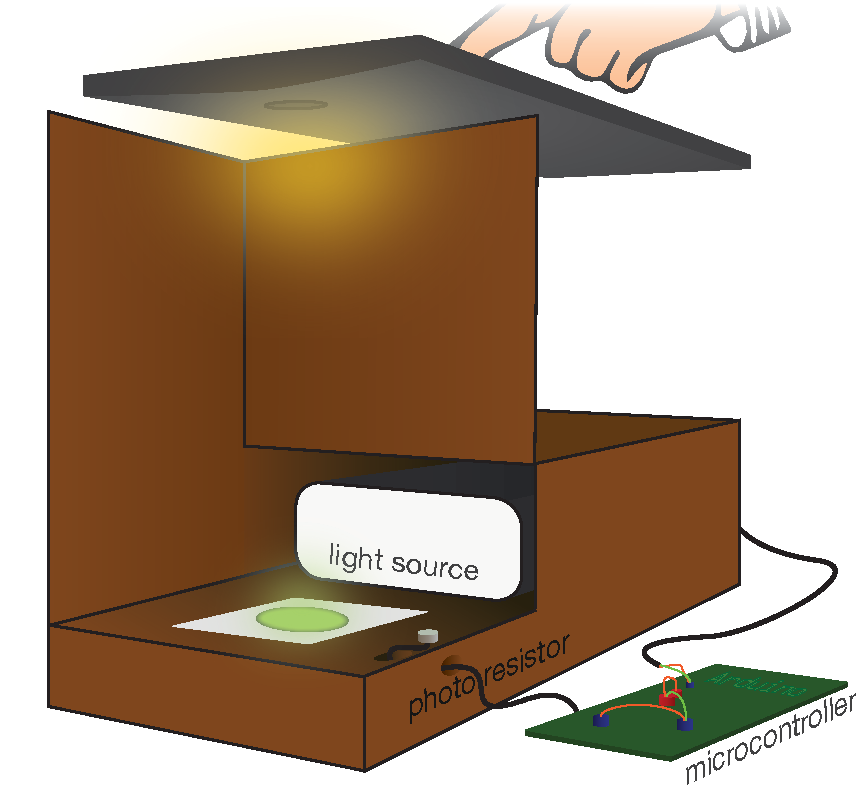
\includegraphics[width=13cm]{images/design_implementation/camera_module.pdf}
\caption{The camera module consists of an external light source, an LDR, and a microcontroller encased in cardboard. \label{figure:camera_module}}
\end{figure}

The actual camera module encloses the taggant fully to protect it from any external light during capture. Pictures of the camera module used in the experiments are included in Appendix \ref{appendix:camera-module}.

The architecture of the module embraces modularity to allow easier prototyping. For example, the light source can be detached from the cardboard casing and the microcontroller allowing different kinds of light sources to be used for the photoexcitation. Moreover, the distance between the taggant and the smartphone can be adjusted by switching the detachable cardboard element (highlighted by the dashed line in Figure \ref{figure:camera_module}) to one of different height. This makes it easy to cater for the variety of different minimum focus distances (MFD) smartphone cameras have.

The microcontroller runs a simple program to monitor the smartphone's torch light. It reads the resistance of the LDR -- the more light the torch light outputs, the lower is the resistance of the LDR. When a sudden increase in the resistance of the LDR is detected (that is, the torch light has turned off) the microcontroller induces voltage into the circuit causing the light source to be triggered. For added safety the light source is isolated from the rest of the circuit by an optocoupler. The schematics of and the program code running on the microcontroller are presented in Appendices \ref{appendix:camera-module-schematics} and \ref{appendix:microcontroller-program}, respectively.

\section{Fingerprint Pipeline}
\label{chapter:fingerprint-pipeline}

The fingerprint pipeline comprises of three distinct steps: the capture of the taggant, analysis of the capture data and matching of the resulting fingerprint. A high level overview of the pipeline is provided in Figure \ref{figure:fingerprint-pipeline}. The following subchapters describe these steps in greater detail.

\begin{figure}[h]
\centering 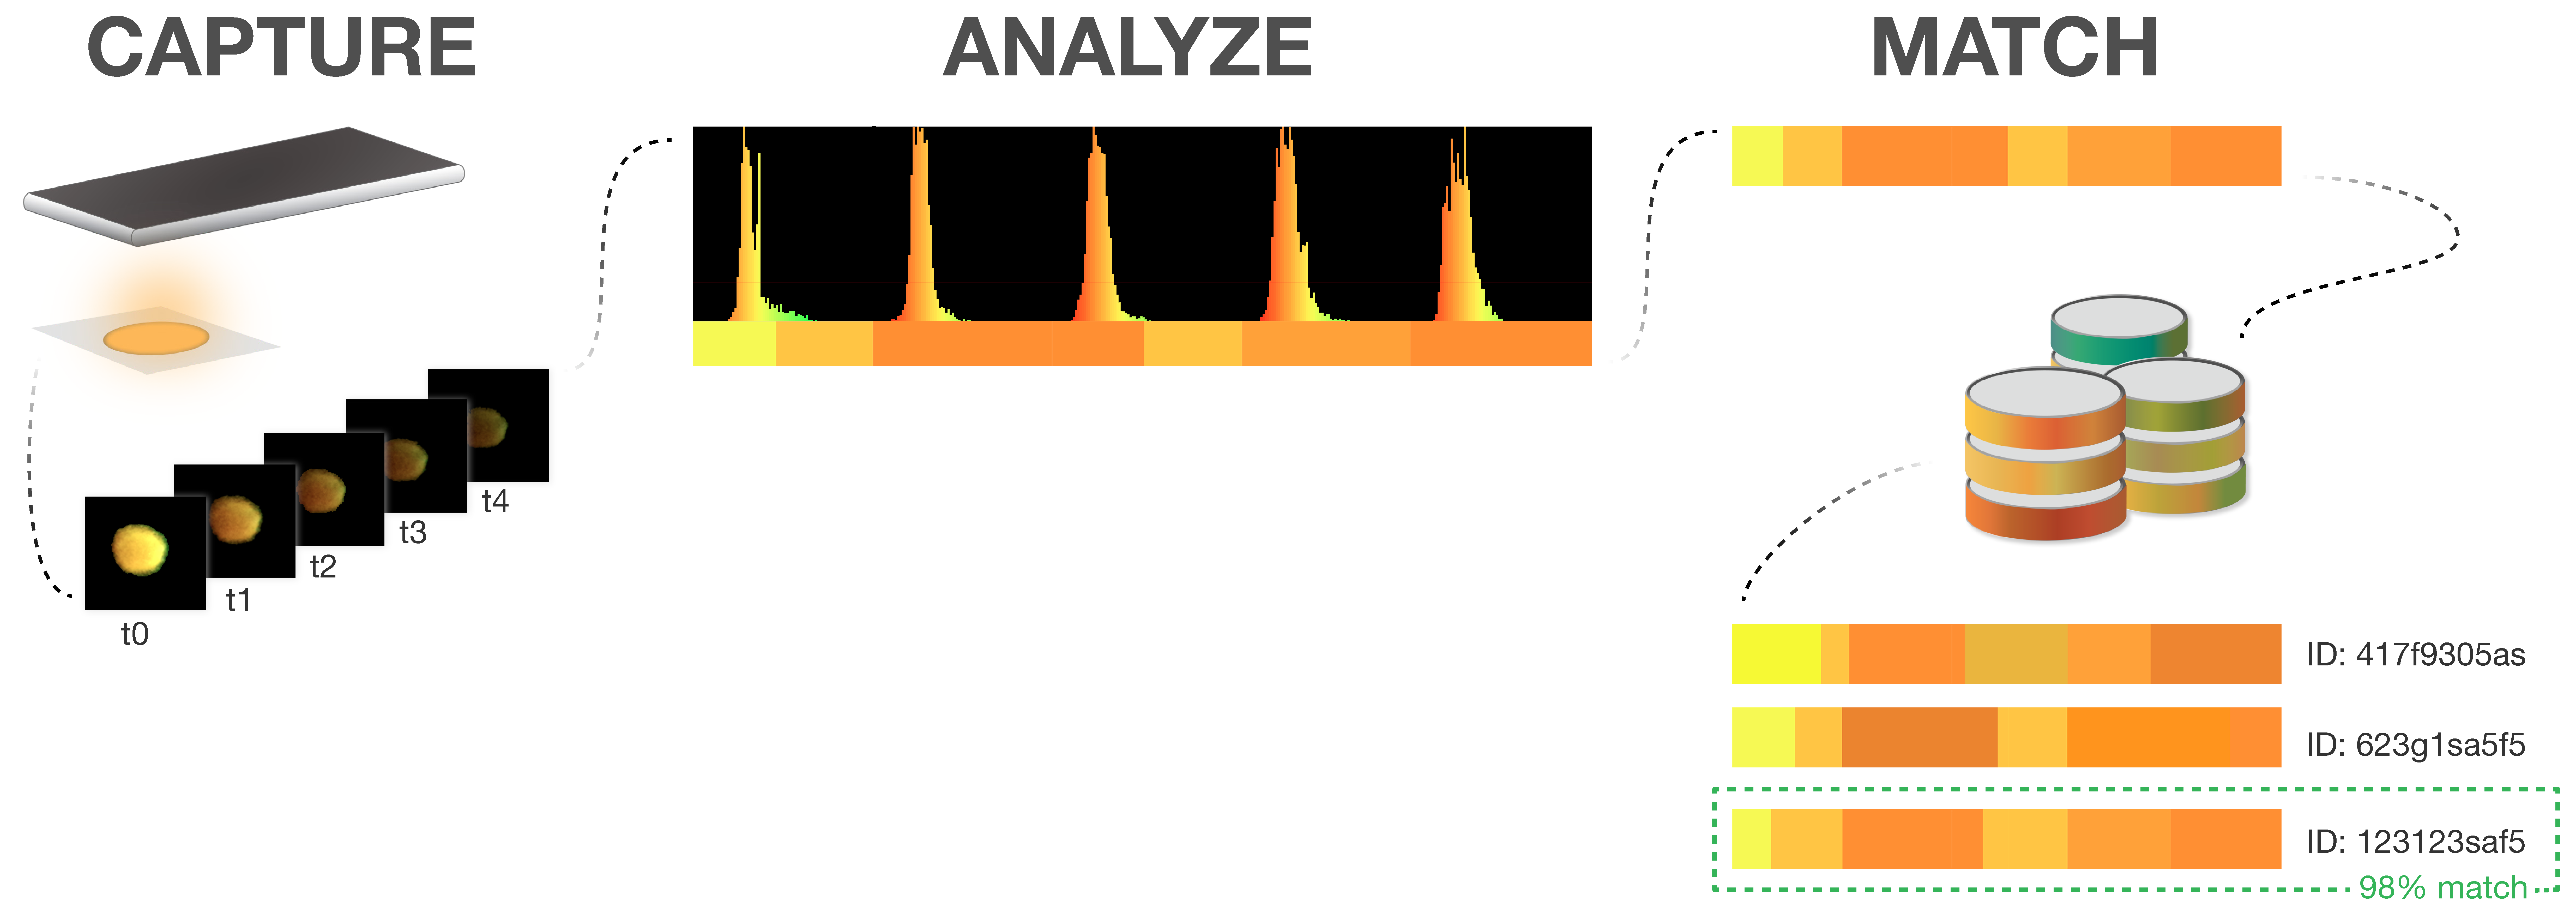
\includegraphics[width=\textwidth,height=\textheight,keepaspectratio=true]{images/design_implementation/fingerprint_pipeline.pdf}
\caption{The fingerprint pipeline. \label{figure:fingerprint-pipeline}}
\end{figure}

\subsection{Taggant Capture}

The taggant is captured as a sequence of images using the parameters introduced in Table \ref{table:camera-parameters}. As illustrated in Figure \ref{figure:camera_module} the smartphone is placed on top of the camera module, which guarantees that the taggant can be isolated from any ambient light, and that the camera will be at the appropriate distance from the taggant -- no closer than the minimum focus distance of the camera. When the user initiates the capture (that is, presses the red capture button as seen in Figure \ref{figure:user_interface}) the camera is first initialized. During initialization the appropriate platform-specific handlers are set and the camera parameters passed via the custom Cordova plugin are applied. After initialization the camera shutter is opened and the torch is toggled to trigger the light source on the camera module. The torch is toggled only after the camera shutter has fully opened to account for any shutter lag.

Once the light source has been triggered the camera application will wait a predefined amount of time (designated by the \emph{delay} parameter in Table \ref{table:camera-parameters}) before capturing the first frame. The duration of the delay is adjusted according to the light source: the longer the light decay of the light source, the longer the capture needs to be delayed to avoid artefacts caused by interference. To track the duration of the delay and to schedule the frames to be captured at a given interval a timer is started. As the first frame is ready to be captured the camera application locks the Auto Exposure (AE), Auto Focus (AF) and Auto White Balance (AWB) controls to guarantee that the camera will use the same exposure, focus and white balance settings for the subsequent frames. Finally, the captured frames are sent to an analyzer component for further processing. The taggant capture process is depicted in Figure \ref{figure:taggant-capture-process}.

\begin{figure}[h]
\centering 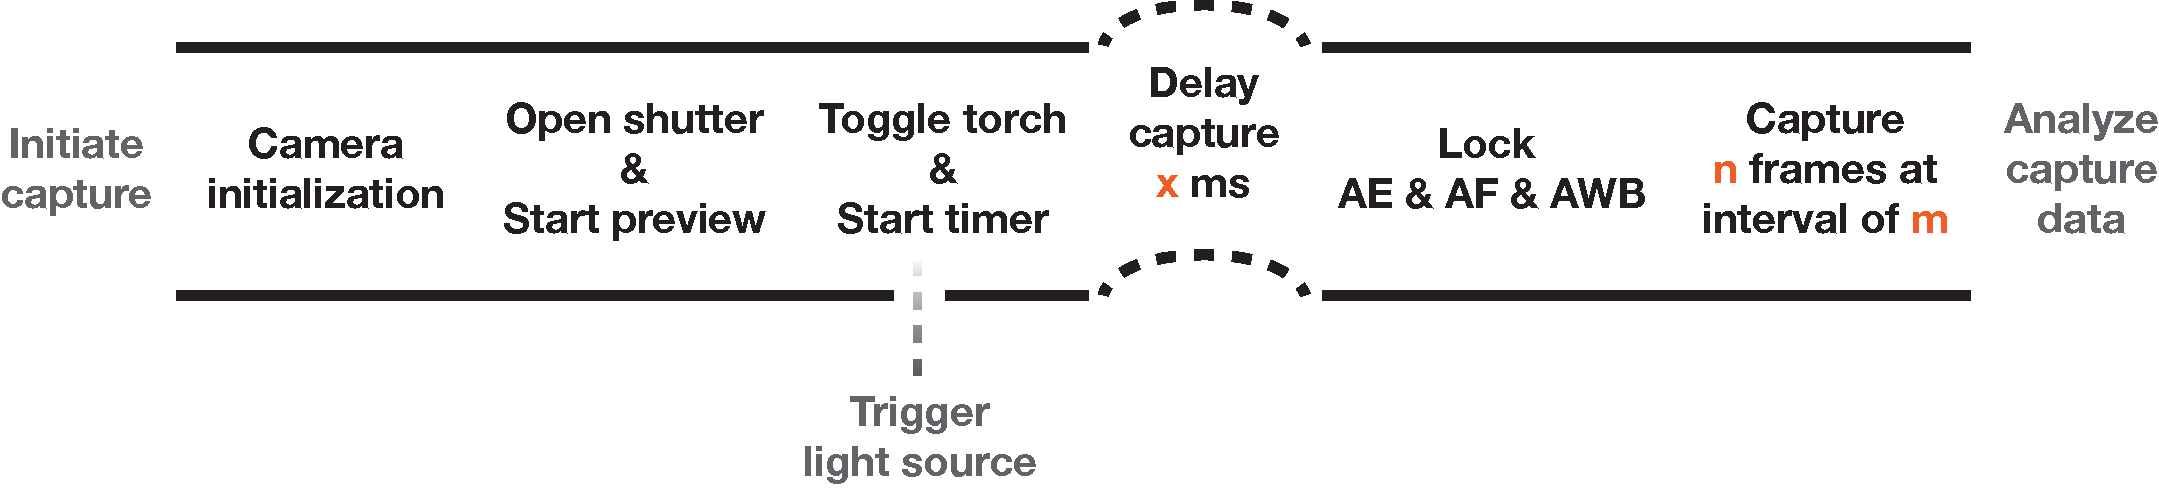
\includegraphics[width=\textwidth,height=\textheight,keepaspectratio=true]{images/design_implementation/capture_process.pdf}
\caption{The taggant capture process. \label{figure:taggant-capture-process}}
\end{figure}

The image sequence is not captured as individual frames, but instead, due to the lack of proper support by the respective APIs, data is captured from the camera's preview feed (refer to Chapter \ref{chapter:discussion} for further discussion). The output from the sensor is read in the YCbCr format. Android encodes the data in the NV21 format whereas Windows Phone uses the NV12 format. The difference between NV21 and NV12 is that the interleave order of Cr and Cb samples is the opposite. The subsampling ratio of these formats is 4:2:0. The rate at which new preview frames were created depended on the Frames Per Second (FPS) supported by the sensor. Higher rate of frames allowed shorter intervals to be used, and thus, the preview FPS was set to the highest possible value (or, range) supported by the platform.

\subsection{Taggant Analysis}

The purpose of the taggant analysis step is to construct a unique fingerprint from the captured frames. The analysis process is illustrated in Figure \ref{figure:taggant-analysis-process}. To prevent blocking the main UI thread and affecting the capture performance each frame is processed (analysed) in its own thread.

\begin{figure}[h]
\centering 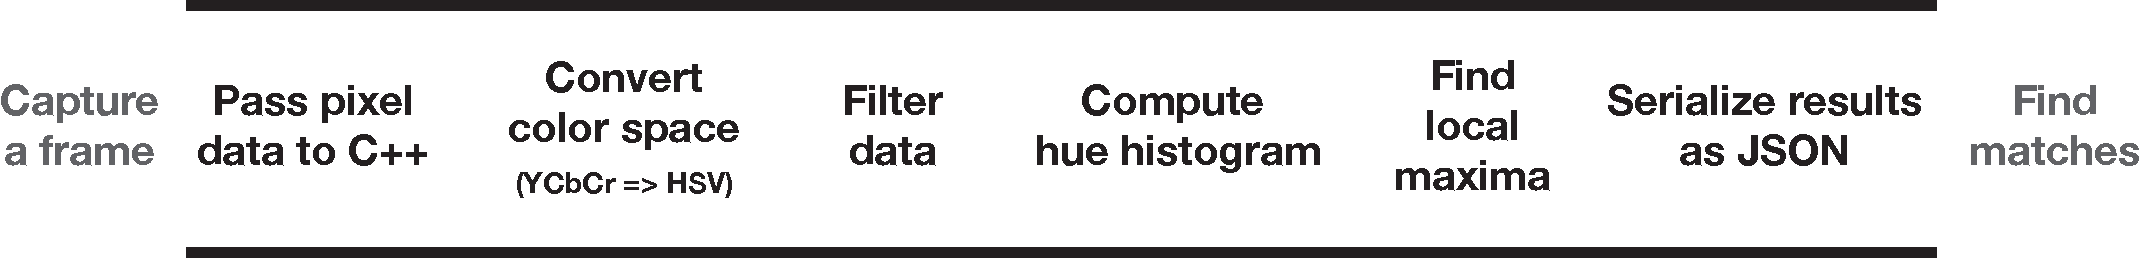
\includegraphics[width=\textwidth,height=\textheight,keepaspectratio=true]{images/design_implementation/analysis_process.pdf}
\caption{The taggant analysis process; each frame is processed in a separate thread to avoid blocking the UI.\label{figure:taggant-analysis-process}}
\end{figure}

Each frame is processed using C++ so that the functionality can be easily reused across platforms. On Android and Windows Phone, calls between the native code and the C/C++ libraries (henceforth referred to as C) are marshalled using the Java Native Interface (JNI) and the C++/CX component extensions, respectively. Another benefit of moving the frame processing to be done in C is the number of robust libraries available for signal processing. The analysis algorithm utilizes the OpenCV\footnote{\url{http://opencv.org/}} open source computer vision library for most of the computations.

The algorithm uses the hue histogram of the captured frame as the basis for the analysis. For each frame the algorithm finds the most dominant hues (hue peaks). The array of peaks computed from the all the frames form a unique \emph{fingerprint}. The taggant analysis consists of multiple processing steps.
Each frame first goes through a color space conversion, where the pixel data is converted from the native YCbCr format to RGB, and then to HSV as per Equation \ref{rgb-to-hsv} utilizing OpenCV's color conversion API. The data is then filtered for noise using binary thresholding, which uses the frame's grayscale information (V channel) to filter pixels that fall outside a certain intensity level (brightness threshold). The thresholding process is illustrated in Figure \ref{figure:binary-thresholding}.

\begin{figure}[h]
\centering 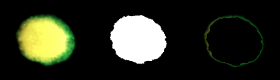
\includegraphics[width=\textwidth,height=\textheight,keepaspectratio=true]{images/design_implementation/binary_thresholding}
\caption{The algorithm uses binary thresholding for noise reduction. The original frame is on the left and the threshold mask is in the middle. The image on the right shows the pixels that would fall outside the threshold.\label{figure:binary-thresholding}}
\end{figure}

The hue histogram can be easily derived from the filtered HSV data using OpenCV's \emph{calcHist} function. The hue peaks are computed from the normalized hue histogram using an open source library called Persistence1D \cite{persistence1d}. The peaks (local maxima) are selected based on a persistence threshold (0-1), which denotes the minimum required delta between a local maxima and minima pair. For example, a persistance threshold of 0.20 would mean that a local minima/maxima pair would only be formed if the delta between the two points were greater than 20\%. Each peak is stored as a 2-dimensional point: $P(hue, intensity)$.

Once all the frames have been captured and their peaks have been computed a fingerprint can be constructed. Given a sequence of \emph{n} frames and a number \emph{m} denoting the most peaks found for a single frame in the sequence the fingerprint can be described as a $n \times m$ matrix. The algorithm encodes the matrix as a JavaScript array and augments it with useful metadata (e.g the capture timestamp of each frame) before sending it to the fingerprint matching algorithm for further processing. An example of the fingerprint output format is provided in Appendix \ref{appendix:fingerprint}.

\subsection{Fingerprint Matching}

In the fingerprint matching step the fingerprint is matched against an existing set of fingerprints (corpus) to find a possible match. The query for fetching the relevant corpus is constructed based on the peak count and average hue of the fingerprint's first sample (frame). The average hue is calculated as a weighted arithmetic mean using the hue intensities as the weights. To allow more flexible queries the value for the peak count and average hue can also be provided as a range. The query format and the databases involded are discussed in more detail in Chapter \ref{chapter:storage-security}.

The fingerprint and the retrieved corpus are given as input to a similarity algorithm. The algortihm ranks the fingerprints in the corpus (candidate fingerprints) against the captured fingerprint (subject fingerprint) based on two simple metrics:

\begin{itemize}
	\item Peak Hue Delta ($P_h$): the difference in peak hue
	\item Peak Intensity Delta ($P_i$): the difference in peak hue intensity
\end{itemize}

The subject fingerprint and a candidate fingerprint are compared frame by frame (sample by sample). That is, the deltas are computed between each $n$th sample of the two fingerprints. The metrics $P_h$ and $P_i$ are given different weights and thresholds. $P_h$ is given more weight and a lower threshold as fingerprints that have dissimilar dominant hues are not likely to be a good match. $P_i$ is given a smaller weight and a higher threshold since slight variations in hue intensities are expected due to noise in the pipeline. The formula used for computing the similarity metrics is given as follows:

\begin{equation}
\label{equation:similarity-metric}
	P_x = \sum \limits_{n=0} { w_x \cdot \max \{\Delta{x_n}-t_x,\ 0\} \cdot d_x^n }
\end{equation}

Where:
\begin{itemize}[label=]
	\item $x$: peak property (e.g. hue or hue intensity)
    \item $P_x$: metric for property $x$ (e.g. $P_h$)
    \item $n$: number of samples in the fingerprint (zero-based)
    \item $w_x$: weight for property $x$
    \item $\Delta{x_n}$: delta between fingerprint samples $n$ for property $x$
    \item $t_x$: delta threshold for property $x$
    \item $d_x$: damping coefficient ($\leq 1$) for property $x$
\end{itemize}

\noindent The purpose of the damping coefficient $d_x$ is to put less emphasis on the latter samples of the fingerprint as it is expected that the first samples are more descriptive of the entire fingerprint.

In order to compute $P_x$ the peaks of the subject and candidate fingerprints have to be paired with each other. The pairing of the peaks becomes an assignment problem where each peak in sample $A_n$ of fingerprint $A$ needs to be paired with a peak in sample $B_n$ of fingerprint $B$ with minimal cost (change in hue). One suitable algorithm for solving the assignment problem for small datasets is the Hungarian algorithm \cite{hungarian_algorithm}. The algorithm takes a $n \times n$ \emph{cost matrix} as input and outputs an $n$ number of $(i, j)$ coordinates (pairs) that represent the minimum cost.

The cost matrix is formed by computing the peak hue deltas ($\Delta{h_n}$) between samples $A_n$ and $B_n$.


The Hungarian algorithm does not, however, solve the \emph{unbalanced assignment problem} where the input is a non-square matrix $n \times m$ ($n \neq m$). This is an issue when samples $A_n$ and $B_n$ have a different number of peaks.

hungarian algorithm (peak count to account for peakless fingerprints)

\begin{figure}[h]
\centering 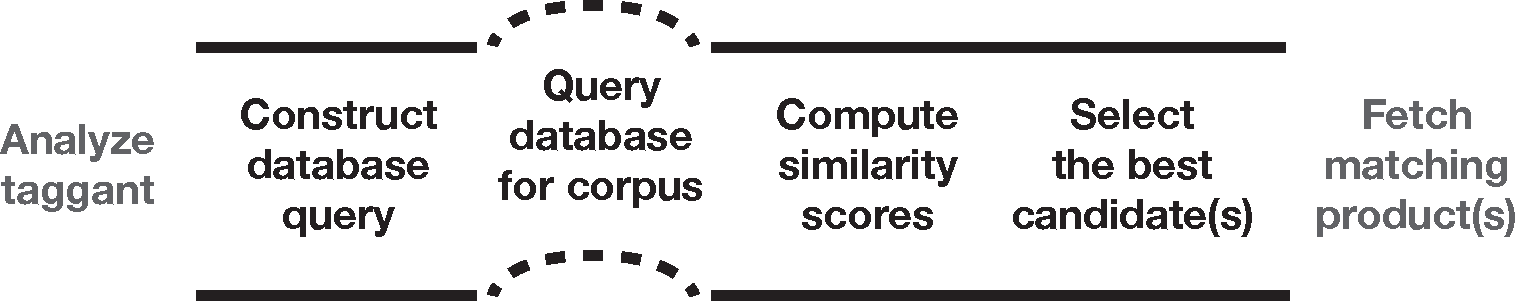
\includegraphics[width=\textwidth,height=\textheight,keepaspectratio=true]{images/design_implementation/matching_process}
\caption{The fingerprint matching process.\label{figure:matching-process}}
\end{figure}

\section{Storage and Security}
\label{chapter:storage-security}

The underlying server back end will consist of a web server and a database to hold the fingerprint data. Optionally, a reverse proxy can be set up in front of the web server to allow static assets to be served to the client without hitting the web server. However, since the application will most likely not include many static assets (images, JS, CSS...) the benefit of this is somewhat minimal. The back end will be implemented using Node.js due to its convenience (author's previous experience and the possibility to re-use the ported spectrum algorithm both in the front and back end). The database will be implemented with MongoDB as it couples well with Node.js and has cross-platform support and an active community.

Eventual consistency (CouchDB) (http://guide.couchdb.org/draft/consistency.html)
Schema flexibility

user management brute force

\end{document}